\documentclass[a4paper]{article}

%% Language and font encodings
\usepackage[english]{babel}
\usepackage[utf8x]{inputenc}
\usepackage[T1]{fontenc}

%% Sets page size and margins
\usepackage[a4paper,top=3cm,bottom=2cm,left=3cm,right=3cm,marginparwidth=1.75cm]{geometry}

%% Useful packages
\usepackage{amsmath}
\usepackage[colorinlistoftodos]{todonotes}
\usepackage[colorlinks=true, allcolors=blue]{hyperref}

\title{Zombie Apocalypse Prep App  }
\author{Jorge Guzman-Nader - (guzmannj)\\ Christa Wright - (wrighch3)\\ Blake Hudson - (hudsonbl)\\ Eric Sisson -  (sissone)\\ Kuan-Yu Lai - (laik)} 

\begin{document}
\maketitle

\includegraphics[width=\textwidth]{index.jpg}
\pagebreak
\tableofcontents
\pagebreak

\section{Product Release}
\subsection{Where can users get the product?}
For now we are locally hosting the website as we update its software. This being said, the website does not have a official URL for users to access. We do have a unofficial URL, http://web.engr.oregonstate.edu/~wrighch3/Zombie/public/, that we use hosted on the OSU servers. Upon accessing the website, there will be no necessary installation processes. Accessing the website is accessing our product.\\

\noindent  The user will run the software by accessing the website. Upon reaching the home page, the user will be interfaced with several options. The options are located in the navigation bar. User stories 1-12 describe how the user will interact with the website. The navigation bar is where the buttons for accessing different features of our website are located. Which those features are described by the user stories. To go into more depth in how the user will access each of these stories or features, is simple user input upon clicking targeted features. A run through of how the system will be utilized by the user will be discussed by the following steps:
\newline
\begin{enumerate}
\item Step 1: Have strong Internet connection
\item Step 2: Use one of the following web browsers to access the website: Chrome, Safari, Internet Explorer or Opera
\item Step 3: Use the following URL https://www.ZombieApocalypse.com/home <---This is our future domain
\item Step 4: For new users skip this step and move to step 5. For recurrent users, view your recent goals by accessing the home page. If not already on the homepage, click the home button on the top of the screen located in the navigation bar. 
\item Step 5: Create a new goal by clicking generate new goals located on the top of the screen(These newly set goals will appear on the homepage).
\item Step 6: Click on the nutrition tab located in the navigation bar on the top of the screen. Enter in numerical values in the spaces provided. 
\item Step 7: Your almost finished using the website! Now you can participate in your own exercise activity. Upon completion of your own goal, click the goals check box on the homepage. 
\item Step 8: Access goal history by pressing the history tab in the navigation bar. This will show recently achieved goals.
\item Step 9: Upon completing goals, the goals provide experience to level up. The experience bar is located on the bottom of the page. 
\item Step 10: Upon leveling up the user will be interfaced with a pop up gif congratulating them on their hard work!
\end{enumerate}

\noindent 
The basic instructions provided above start the user out with how to use the website. It is necessary for the user to have access to a computer and Internet in order for the user to have access to our product.  


\section{User Story}
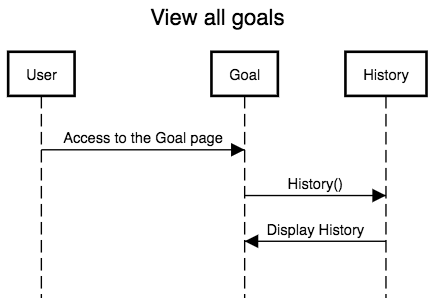
\includegraphics[width=\textwidth]{View_all_goals.png} 
\newline
\newline
\newline
\begin{itemize}
  \item Christa and Eric are working on this feature.
  \item We haven't found any problem yet since the feature are still in developing step.
  \item The running time of the task should be last then 3 seconds and the developing time should be approximately 3 days.
  \item The current status are developing.
  \item The functionality of the page still needs to be done.
  \item Yes, the diagram is useful since it helps us understand the relation between each feature.
  \item Currently we feel like the diagrams are good for us.
\end{itemize}
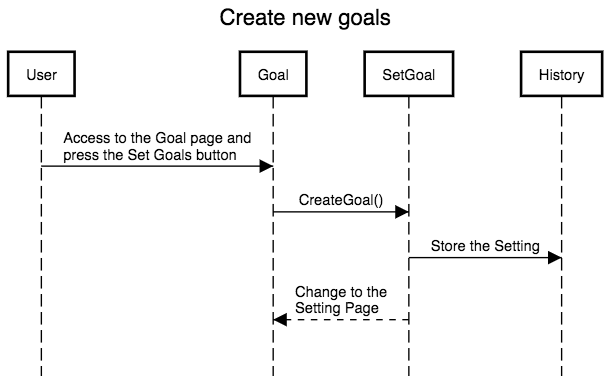
\includegraphics[width=\textwidth]{Create_new_goals.png}

\begin{itemize}
	\item Eric is working on this feature. 
	\item We haven't found any problem yet.
    \item The running time of the task should be last then 1 seconds and the developing time should be approximately 2 days.
    \item The current status are developing.
  \item The functionality of the page still needs to be done.
  \item Yes, the diagram is useful since it helps us understand the relation between each feature.
  \item Currently we feel like the diagrams are good for us.
\end{itemize}

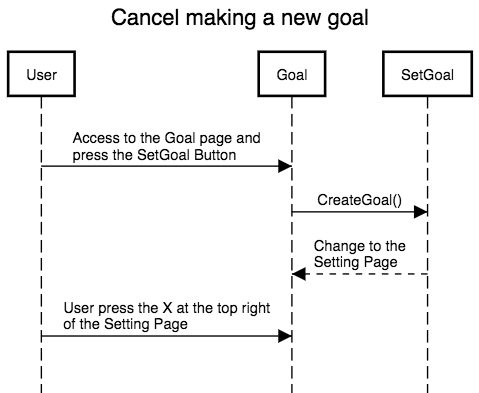
\includegraphics[width=\textwidth]{Cancel_making_a_new_goal.png}
\begin{itemize}
	\item Blake is working on this feature. 
	\item We haven't found any problem yet.
    \item The running time of the task should be last then 1 seconds and the developing time should be approximately 2 days.
    \item The current status are developing.
  \item The functionality of the page still needs to be done.
  \item Yes, the diagram is useful since it helps us understand the relation between each feature.
  \item Currently we feel like the diagrams are good for us.
\end{itemize}
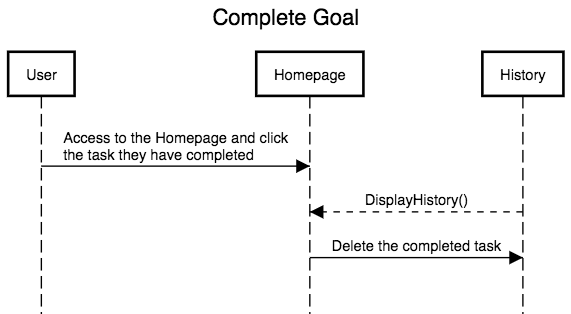
\includegraphics[width=\textwidth, height=8cm]{Complete_Goal.png}
\begin{itemize}
	\item Christa is working on this feature. 
	\item We haven't found any problem yet.
    \item The running time of the task should be last then 1 seconds and the developing time should be approximately 2 days.
    \item The current status are developing.
  \item The functionality of the page still needs to be done.
  \item Yes, the diagram is useful since it helps us understand the relation between each feature.
  \item Currently we feel like the diagrams are good for us.
\end{itemize}
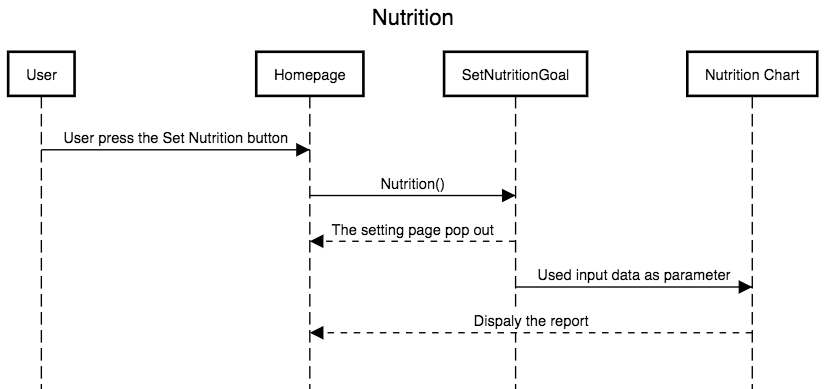
\includegraphics[width=\textwidth, height=8 cm]{Nutrition.png}
\begin{itemize}
	\item Jorge is working on this feature. 
	\item We haven't found any problem yet.
    \item The running time of the task should be last then 3 seconds and the developing time should be approximately 5 days.
    \item The current status are developing.
  \item The functionality of the page still needs to be done.
  \item Yes, the diagram is useful since it helps us understand the relation between each feature.
  \item Currently we feel like the diagrams are good for us.
\end{itemize}
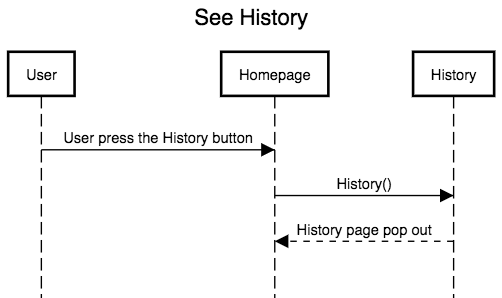
\includegraphics[width=\textwidth, height=8 cm]{See_History.png}
\newline
\begin{itemize}
	\item York is working on this feature. 
	\item We haven't found any problem yet.
    \item The running time of the task should be last then 3 seconds and the developing time should be approximately 4 days.
    \item The current status are developing.
  \item The functionality of the page.
  \item Yes, the diagram is useful since it helps us understand the relation between each feature.
  \item Currently we feel like the diagrams are good for us.
\end{itemize}

\section{Design changes and rationale}
The customers have been easy to get a hold of and respond quickly to questions. They provide insightful information on how the Zombie Prep App should look, and offer ideas on how to implement it. 
\newline
\newline
We asked the customers about the hosting of the web application and  viable options for  implementing our server. The customer agreed in hosting the web application either in the school server or github, depending of convenience and ease of use. After further discussion and some research, the best options seems to be hosting the web application on Oregon State University's Engineering web server that the students have access to. 
\newline
\newline
We decided to use the school's server, we will need to make a database using php, and we will  re-purpose some of our features to match this new framework, this increases the complexity of the project do to the new learning curve, but still viable to implement in the scheduled time. 
\newline
\newline
We also asked the customer about the user interface functionalities, specifically about the goals button, the customers propose a layout that was more user friendly and intuitive that the previously made. We modified the code for the front end of our goals tracking feature so it matches the new version. 
\newline
\newline
We decided that when making the goals, instead of taking the user to a new page we would just make a modal that would go over the goals page. 
\newline
\newline
The customer also suggested making the web page accessible to make it easier for people who are colorblind or who are visually impaired, such as not seeing well. Due to HTML having pre - built functionality already in it, the group won't have to put in much more effort to make the web application accessible to users. The bootstrap that the page already uses will also make it accessible when the page is zoomed in. The user would be able to tab through links easily with the HTML that the page uses, and will be able to tab between the forums as they enter information into it. 
\newline
\newline
We also re-assigned tasks to different group members, based in how our work flow has changed and the expertises of our members with the new tools implemented in our page. The scheduling of each of our user stories also changed, because of the implementation of the new database that is fundamental for many of the other features. 


\section{Tests}
Testing allows the Zombie Apocalypse Prep Application to meet quality expectations, and ensures that the system won't run into bugs while in use. The web application will need to test user validation to ensure the user receives the expected feedback. Additionally, we will be testing to verify the system is also usable and acceptable by the customer's standards.  Without the testing, the user may receive results that they were not expecting, or the customer may not receive the product they wanted. 
\newline
\newline
There are two main user input sections in the web app; where the user makes their goals, and where the user inputs their nutritional information. These two forums will require a unit test that validates what the user has inputed into the text box. The goals form is a little bit different from the nutrition form. The goals will require the user to select an option from two lists for the goal to be processed. Without each list having something selected from it, the goal can't be created, because it would need an activity and an integer to proceed. The integer would act as either a distance or time, depending on the activity selected.  For a quick test we may do some random testing, to make sure that the scripts we have written are checking the input correctly. This will just be to check that the program is not accepting an unrealistic input, such as negative twenty pounds in the nutrition section. Later more advanced verification tests will be written to ensure quality.  Despite this section not being completely polished out, the verification will be implemented shortly. 
\newline
\newline
The main user story is the same as the previous paragraph; the user should be able to enter valid user data and expect a reasonable output based on what they have entered. Testing this will involve input validation. 
\newline
\newline
For debugging our web application, we will be using the console.log() JavaScript command. This prints out to the developer screen anytime we call it in our code. This is how we will check for user click events, input handling, etc.. The use of this will give us instant feedback while using the website itself. Any cases where the logged output of a section we are testing will tell us that the code is not validating the user commands correctly. This is where we can then go into the code and change what is needed to validate user commands. It is a common debugging method used by web developers. 
\newline
\newline
The last test, we will do Acceptance Testing. This will be the first step in our testing process, and it will follow an ad hoc method. We will check to see if the software meets the customer's requirements. We will access if it suitable to be delivered by making sure it matches the stake holder's requirements.  To test for this, we will run through the program to make sure it works for a demonstration. 
\newline
\newline
Another aspect of testing would be checking to make sure the website is usable. If the website is not intuitive and easy to learn, then the website will fail in it's goal; creating a usable goal tracking application. To see if the website is usable, we will run through various usability heuristics to ensure it meets quality expectations. Part of the testing will ensure that the user's options are visible, like the buttons to make a new goal. The user would have some constraints, such as the information entered in the nutrition area would need to be kept with in reason - such as preventing someone from entering a negative weight.  
\newline
\newline
Finally we will make a regression test, for every feature that we change or implement to be sure that each unit and the whole system still behave as we expect it to behave.


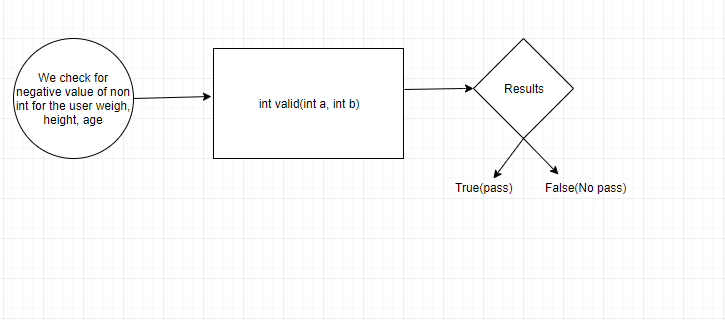
\includegraphics[width=\textwidth, height=8 cm]{nuberInput.png}
This test checks if the input for the nutrition unit is negative or other thing than an integer. It has a value a which if is not bigger than zero throw a false, else is true and the test ends.
The other parameter b checks if the value is an int and return true if so, if not it return a false .
\newline
\newline
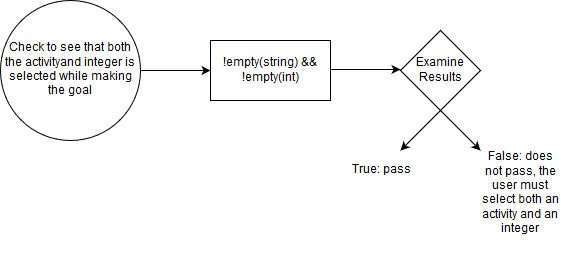
\includegraphics[width=\textwidth, height=8cm]{goals.png}
This checks to see if the input for the goals form is entered correctly. That is, the user must select both an activity and an integer, which would either represent a distance or a certain amount of time that the user will do the activity for. Without both of these selected, the goal would not be able to be made correctly, thus allowing the user to create a goal successful. 

\section{Meeting Report}

\subsection{Schedule for next week} 
For the next week we plan to work in :\\	

\noindent Implementing the hosting inside the school server, this will be done as late as  03/04\\
\noindent Re-format the create new goals UI will be done 03/11\\
\noindent Cancel making a goal will be done this 03/11\\
\noindent Mark a goals as completed in the UI 03/11\\
\noindent Have functional parts of the nutrition feature in the page 03/11\\
\noindent Implement the history feature by using the database 03/15\\

\subsection{Progress this week }
We implemented great part of the main framework for the application to live in, we did this using html/css.\\
\noindent We plan how to tackle possible future constrains that we will encounter while implementing the more interactive features., such as how to validate the user input and prevent invalid inputs to be used, how to make the webpage more easy navigable by the user, how to implement the server or host the page in an efficient way, and how to preform the nutrition calculation based in real  medical and biochemical data.
\subsection{Plans and goals for next week}
Next week we plant to:\\
Implementing the hosting server :We plan to use the server and database that the school provides to host our application, the difficulty in this is change our application to make it work well with php scrip.\\

\noindent Re-format the create new goals UI: We need to add the new designs  to the already created framework and show that it works as intended.\\

\noindent Cancel making a goal will: We hope to be able to implement this feature next week, the feature will make the user able to cancel a goal that has been made by error or just because the user want to.\\

\noindent Mark a goals as completed: We plan to implement a "label" or other visual feature that indicates the user when a goal has been completed.\\

\noindent Have functional parts of the nutrition feature: We want to at least be able to run calculations for macro-nutrients in the application and that the application return a graph of the nutrients required.\\

\noindent Implement the history feature by using the database: We hope to have this completed in time, because non of our team member have deep background in databases this feature could be passed to another week, but if we complete it on time, we plan to make the database return a list of the competed goals  and that the user can check them at he/she discretion.\\

\subsection{Team member contribution}

Christa made most of the framework and implemented the UI, she also helped planning how to use the hosting  of the page. Eric added partial functionalities for the goals making feature, Blake help with the writing and documentation of the software, York help with the  database and diagrams, Jorge helped with documentation, testing and the nutrition feature.\\

\subsection{Customer meeting }
Our customers were able to meet and direct the efforts of this project toward a feasible goal. Our customer were also responsible for most of the code written this week.

\end{document}